% ------------------------------------------------------------------------------
% TYPO3 CMS 8.6 - What's New - Chapter "Backend User Interface" (Serbian Version)
%
% @author	Michael Schams <schams.net>
% @license	Creative Commons BY-NC-SA 3.0
% @link		http://typo3.org/download/release-notes/whats-new/
% @language	English
% ------------------------------------------------------------------------------
% LTXE-CHAPTER-UID:		07b25346-95b1df21-a6ebe09a-49f53f41
% LTXE-CHAPTER-NAME:	Backend User Interface
% ------------------------------------------------------------------------------

\section{Backend User Interface}
\begin{frame}[fragile]
	\frametitle{Backend User Interface}

	\begin{center}\huge{Chapter 1:}\end{center}
	\begin{center}\huge{\color{typo3darkgrey}\textbf{Backend User Interface}}\end{center}

\end{frame}

% ------------------------------------------------------------------------------
% LTXE-SLIDE-START
% LTXE-SLIDE-UID:		27fe5677-7998aeff-2161886f-e5835be1
% LTXE-SLIDE-ORIGIN:	4141a9cc-46da51df-9dd87a8b-9b15ac29 English
% LTXE-SLIDE-TITLE:		#12211: Scheduler Page Browser
% LTXE-SLIDE-REFERENCE:	!Feature: #12211 - Usability: Scheduler provide page browser to choose start page
% ------------------------------------------------------------------------------
\begin{frame}[fragile]
	\frametitle{Backend User Interface}
	\framesubtitle{Scheduler Page Browser}

	To improve the usability of the \textbf{EXT:linkvalidator} scheduler task,
	the page browser was added to select the start page.

	\begin{figure}\vspace{-0.2cm}
		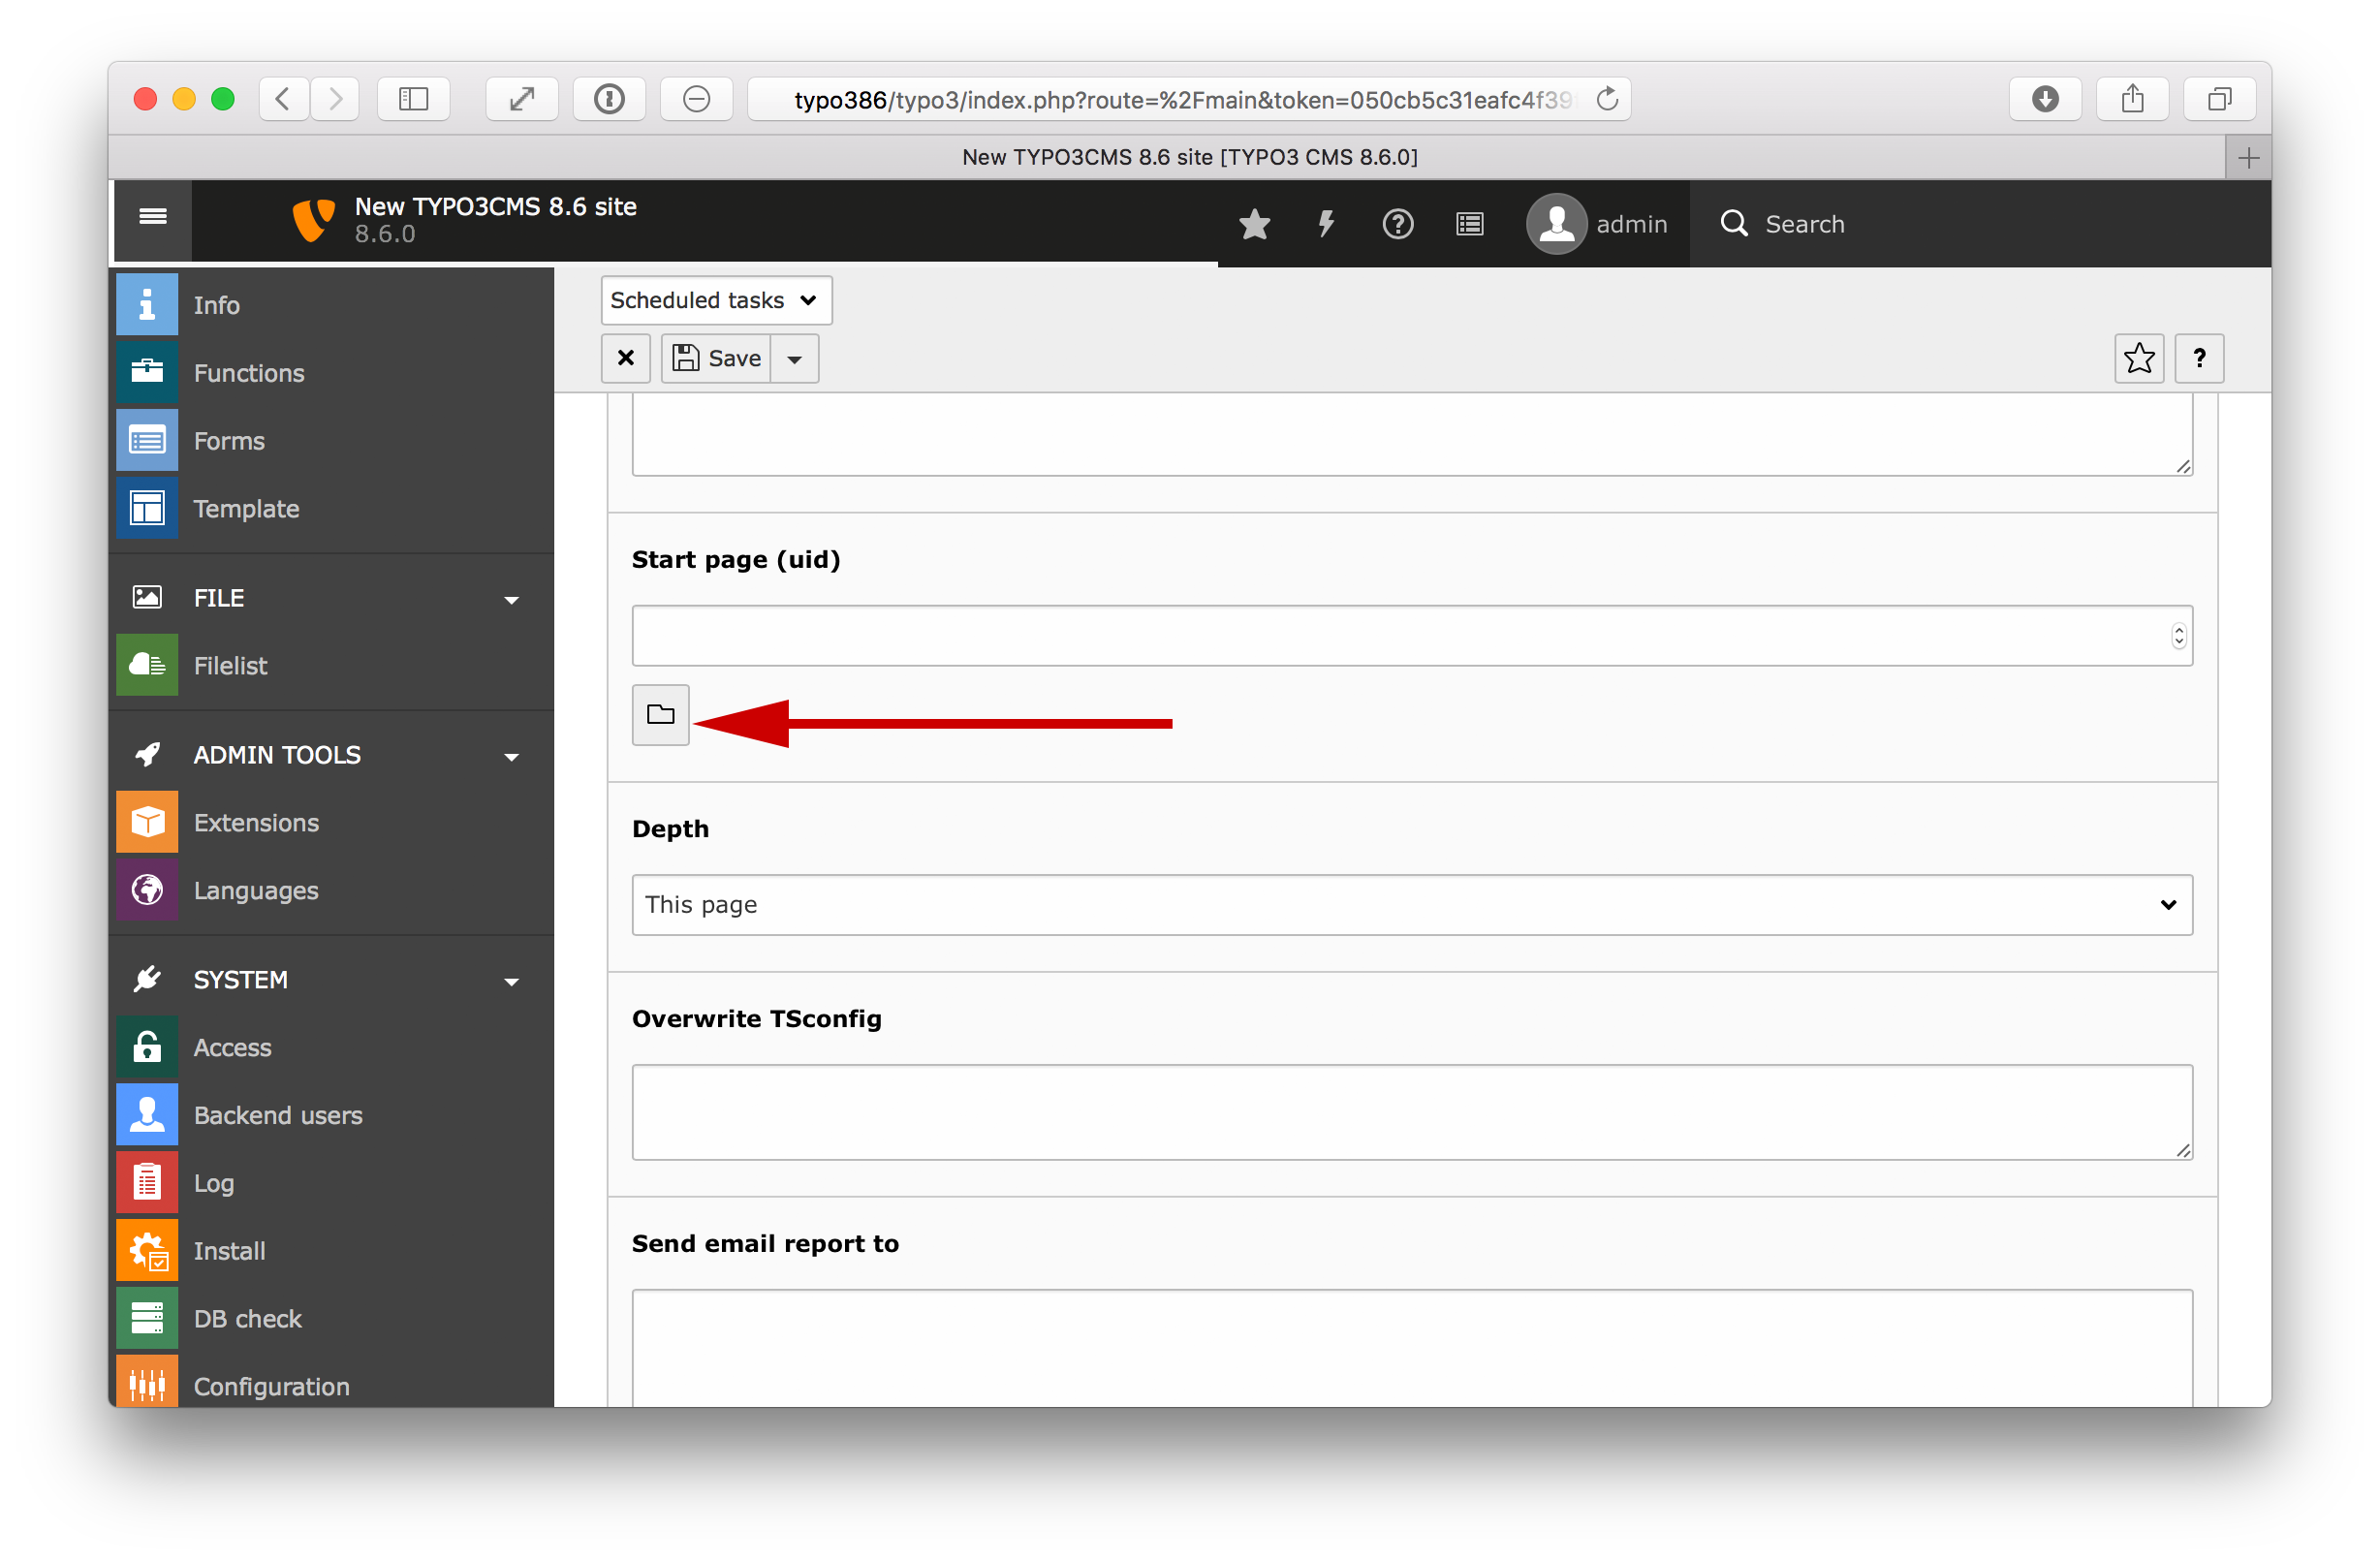
\includegraphics[width=0.67\linewidth]{BackendUserInterface/12211.png}
	\end{figure}

\end{frame}

% ------------------------------------------------------------------------------
% LTXE-SLIDE-START
% LTXE-SLIDE-UID:		08cb86a4-29caed86-57a340a8-a5576a6a
% LTXE-SLIDE-ORIGIN:	f924be39-75ae40d9-ba00f0a8-3a6de040 English
% LTXE-SLIDE-TITLE:		#45537: Manually executed tasks
% LTXE-SLIDE-REFERENCE:	!Feature: #45537 - Run manually executed tasks on next cron-run
% ------------------------------------------------------------------------------
\begin{frame}[fragile]
	\frametitle{Backend User Interface}
	\framesubtitle{Run Manually Executed Tasks on Next Cron-run}

	\begin{columns}[T]
		\begin{column}{0.3\textwidth}
			There is a new action icon to mark a task to be run by cron. Also a new button
			"Execute selected tasks on next cron job" has been added to mark all selected actions
			to be run by next cron job.
		\end{column}

		\begin{column}{0.7\textwidth}
			\begin{figure}\vspace{-0.6cm}
				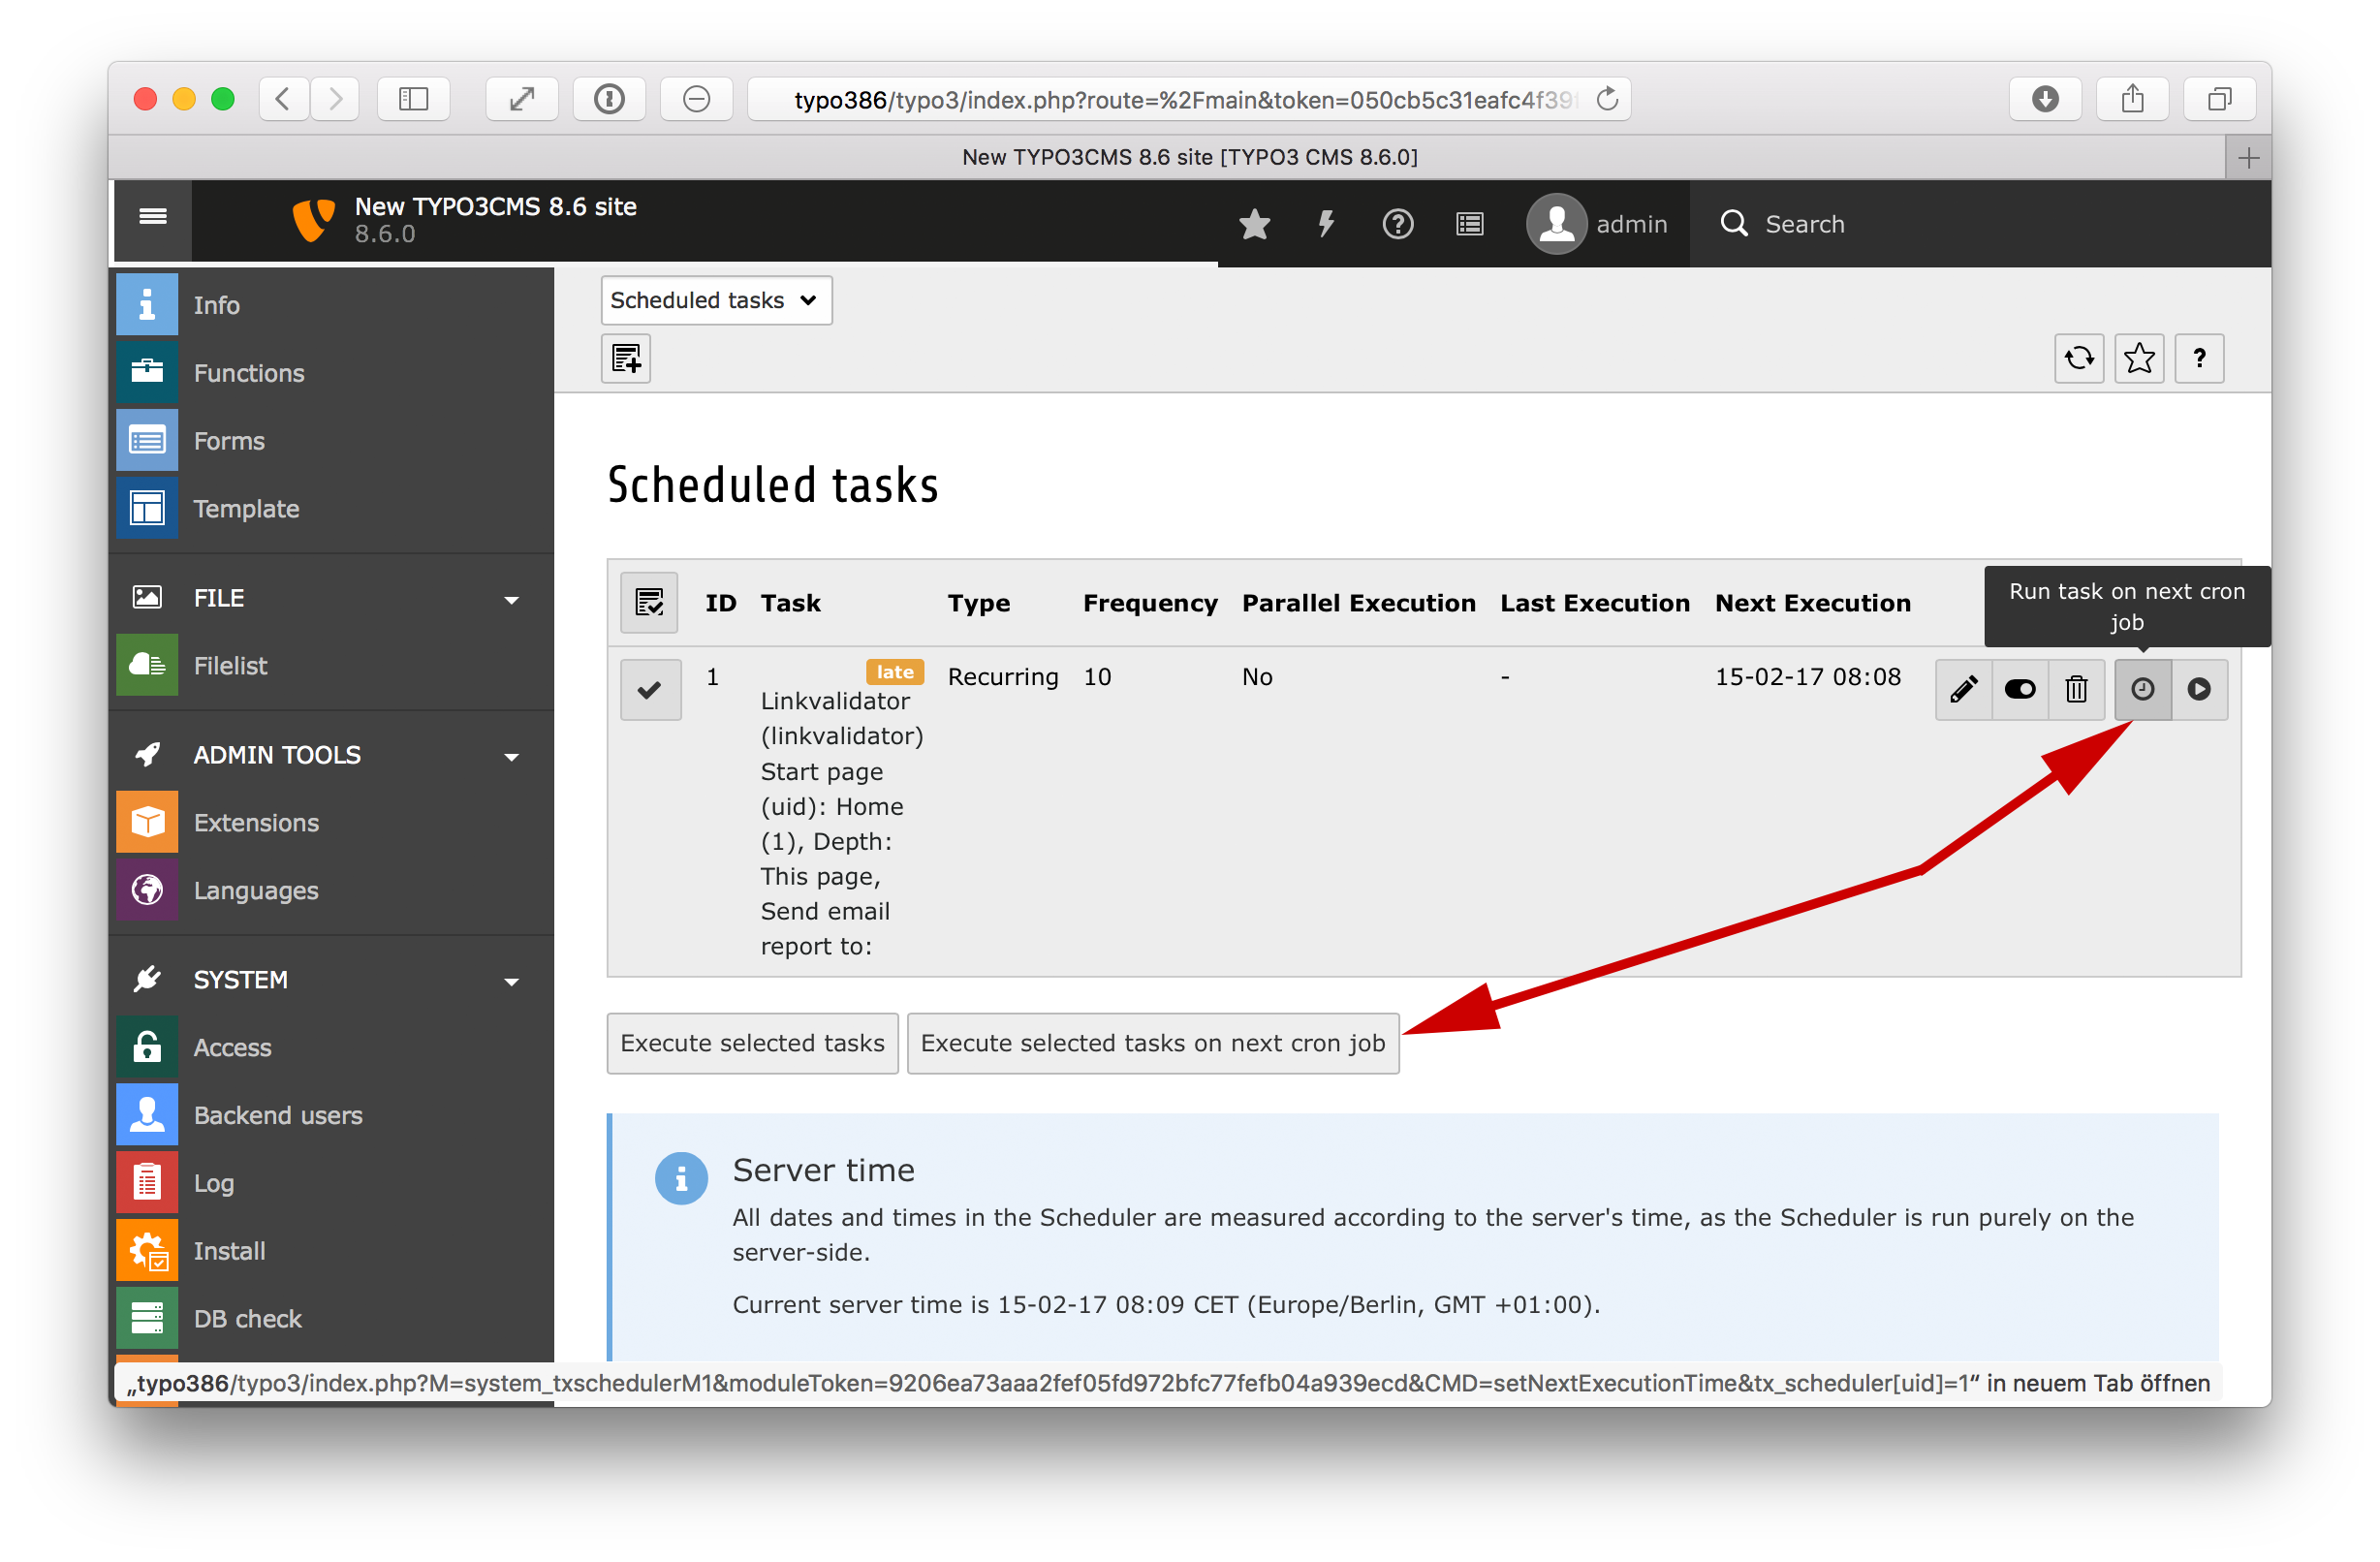
\includegraphics[width=0.99\linewidth]{BackendUserInterface/45537.png}
			\end{figure}
		\end{column}
	\end{columns}

\end{frame}

% ------------------------------------------------------------------------------
% LTXE-SLIDE-START
% LTXE-SLIDE-UID:		3c7ec0f7-a7f72aea-e89b17a8-16821d1f
% LTXE-SLIDE-ORIGIN:	b6d6054e-21291d35-479a0095-a6e82a4f English
% LTXE-SLIDE-TITLE:		#47135: Paste Icon and Modal
% LTXE-SLIDE-REFERENCE:	!Feature: #51291 - Synchronized field values in localized records
% ------------------------------------------------------------------------------
\begin{frame}[fragile]
	\frametitle{Backend User Interface}
	\framesubtitle{Paste Icons and Modal}

	As soon as the normal clipboard contains an item, a single paste icon becomes available
	in the page module. When the user clicks on the icon, a modal pops up to have the user
	confirm the action.

	\begin{figure}\vspace{-0.2cm}
		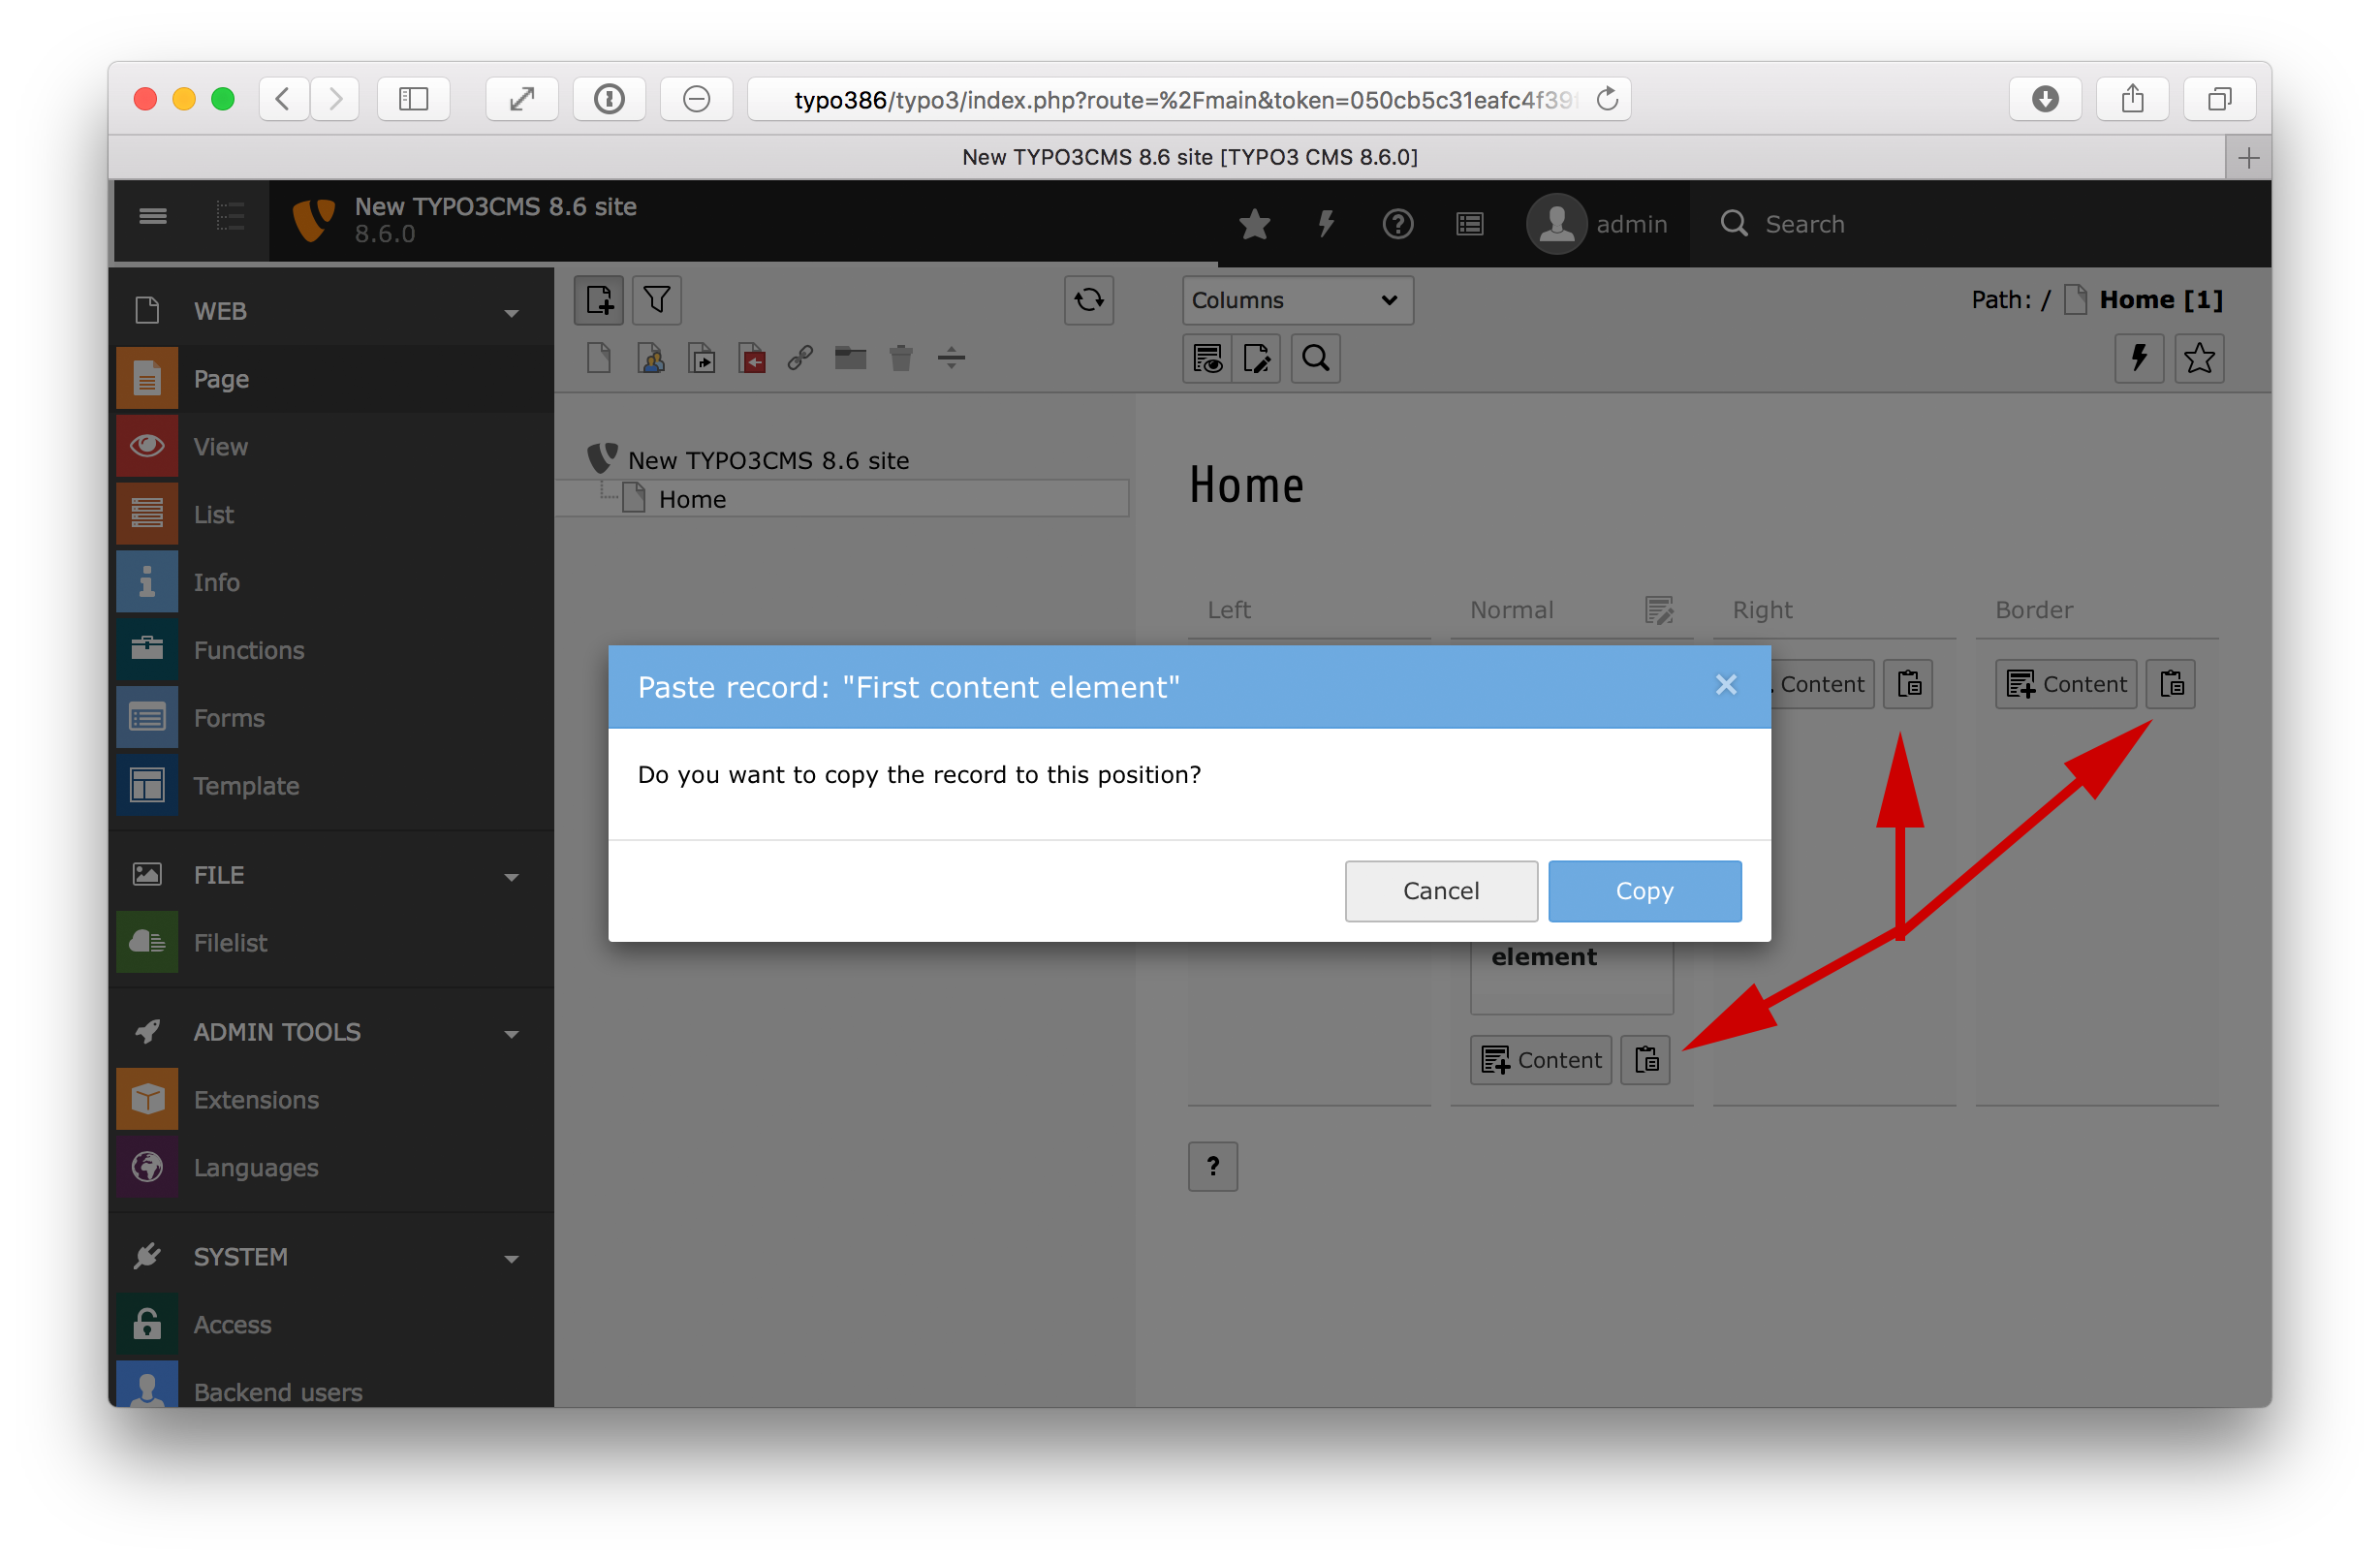
\includegraphics[width=0.63\linewidth]{BackendUserInterface/47135.png}
	\end{figure}

\end{frame}

% ------------------------------------------------------------------------------
% LTXE-SLIDE-START
% LTXE-SLIDE-UID:		ce21c798-b42bd93c-f46b8ddd-5b94032d
% LTXE-SLIDE-ORIGIN:	b31e455f-fce042ed-e3670436-9e72983c English
% LTXE-SLIDE-TITLE:		#67243: Folding of Scheduler Task Groups
% LTXE-SLIDE-REFERENCE:	!Feature: #67243 - Implement folding of scheduler task groups
% ------------------------------------------------------------------------------
\begin{frame}[fragile]
	\frametitle{Backend User Interface}
	\framesubtitle{Folding of Scheduler Task Groups}

	When task groups are used, the tasks are displayed grouped in the list of tasks.
	Clicking on the row with the group title hides or shows the tasks of the group now.

	\begin{figure}\vspace{-0.3cm}
		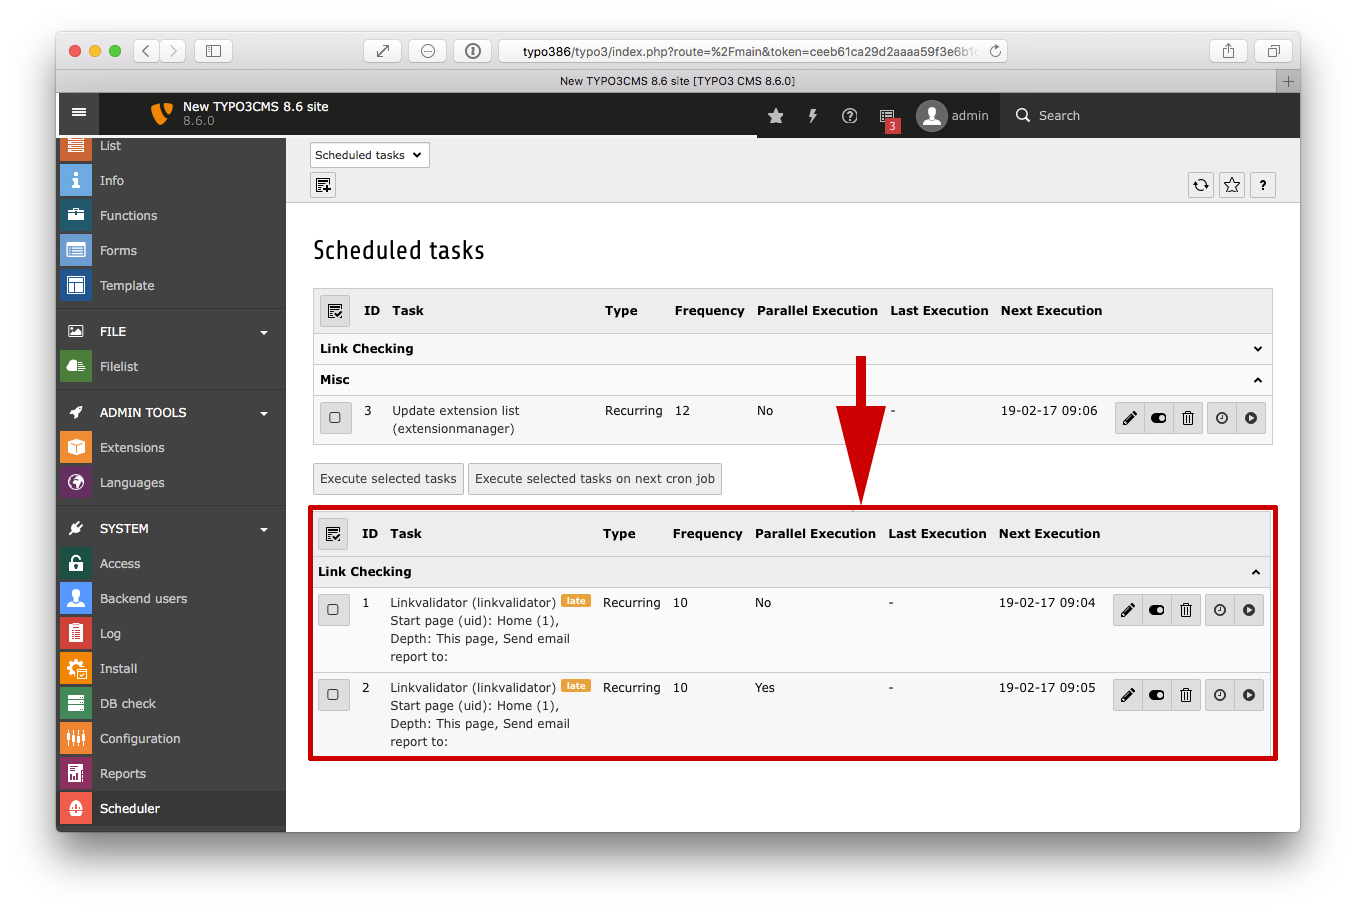
\includegraphics[width=0.60\linewidth]{BackendUserInterface/67243.png}
	\end{figure}

\end{frame}

% ------------------------------------------------------------------------------
% LTXE-SLIDE-START
% LTXE-SLIDE-UID:		73f9b847-af3fdd0a-f02d1884-2e750555
% LTXE-SLIDE-ORIGIN:	14fe5a0b-2a22a6ce-325b5de1-ef26ce50 English
% LTXE-SLIDE-TITLE:		#69572: Page Module Notice
% LTXE-SLIDE-REFERENCE:	!Feature: #69572 - Page module Notice "Content is also shown on:"
% ------------------------------------------------------------------------------
\begin{frame}[fragile]
	\frametitle{Backend User Interface}
	\framesubtitle{Page Module Notice "Content is also shown on"}

	\begin{columns}[T]
		\begin{column}{.3\textwidth}
			When page content is inherited from a different page via "Show content from page",
			a notice is displayed on the page that is pulling in content to a different page.
		\end{column}

		\begin{column}{.7\textwidth}
			\begin{figure}\vspace*{-0.6cm}
				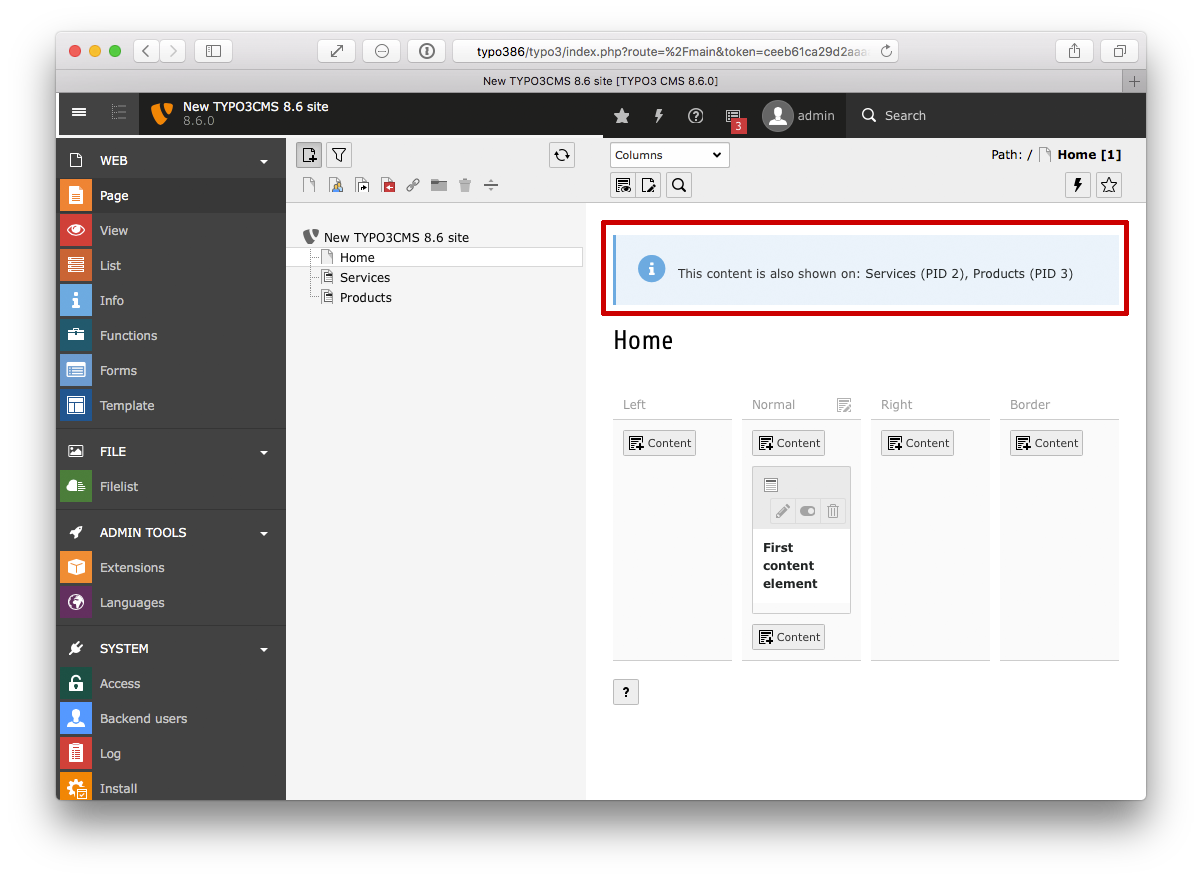
\includegraphics[width=\linewidth]{BackendUserInterface/69572.png}
			\end{figure}
		\end{column}
	\end{columns}

\end{frame}

% ------------------------------------------------------------------------------
% LTXE-SLIDE-START
% LTXE-SLIDE-UID:		c83663fa-2e7239fe-f713beb7-9393f4ff
% LTXE-SLIDE-ORIGIN:	23a4baef-462e7d0c-c8cd4cfc-9dac1f99 English
% LTXE-SLIDE-TITLE:		#75880: Image Manipulation - Multiple Cropping Variants
% LTXE-SLIDE-REFERENCE:	!Feature: #75880 - Implement multiple cropping variants in image manipulation tool
% ------------------------------------------------------------------------------
\begin{frame}[fragile]
	\frametitle{Backend User Interface}
	\framesubtitle{Image Manipulation - Multiple Cropping Variants}

	The Image-Manipulation tool is now capable of handling multiple crop variants (if configured).
	Users can also select a focus area, which is always inside the crop area and mark the area
	in the image which must be visible % -- beware of text flow here, it continues in the column

	\begin{columns}[T]
		\begin{column}{.35\textwidth}
			for the image to transport its meaning.
			To give editors a hint which area of the image is used by other DOM-Elements like headlines,
			when selecting a crop area, it is possible to define multiple so called cover areas.
		\end{column}

		\begin{column}{.65\textwidth}
			\begin{figure}\vspace*{-0.6cm}
				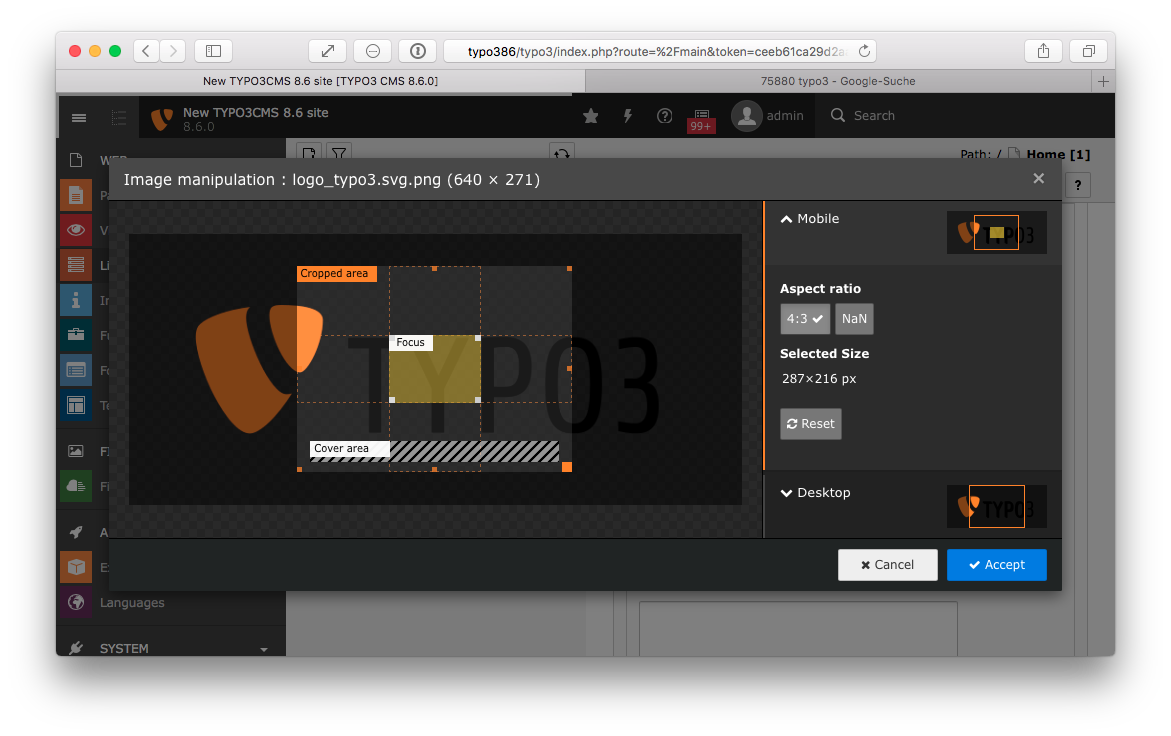
\includegraphics[width=0.99\linewidth]{BackendUserInterface/75880.png}
			\end{figure}
		\end{column}
	\end{columns}

\end{frame}

% ------------------------------------------------------------------------------
% LTXE-SLIDE-START
% LTXE-SLIDE-UID:		190c2c60-c95b9272-0f608d56-a2667d4a
% LTXE-SLIDE-ORIGIN:	8f2f695d-f5c6a8bf-5700cf34-d6389ce8 English
% LTXE-SLIDE-TITLE:		#79235: Delete Similar Errors (sys_log)
% LTXE-SLIDE-REFERENCE:	!Feature: #79235 - Add button to delete similar errors from sys_log
% ------------------------------------------------------------------------------
\begin{frame}[fragile]
	\frametitle{Backend User Interface}
	\framesubtitle{Delete Similar Errors from \texttt{sys\_log}}

	The log module of TYPO3 now shows a button to delete multiple errors at once based on the
	\texttt{details} field of the \texttt{sys\_log} table. This comes in handy when you fixed
	an error that spammed the log before.

	\begin{figure}\vspace{-0.2cm}
		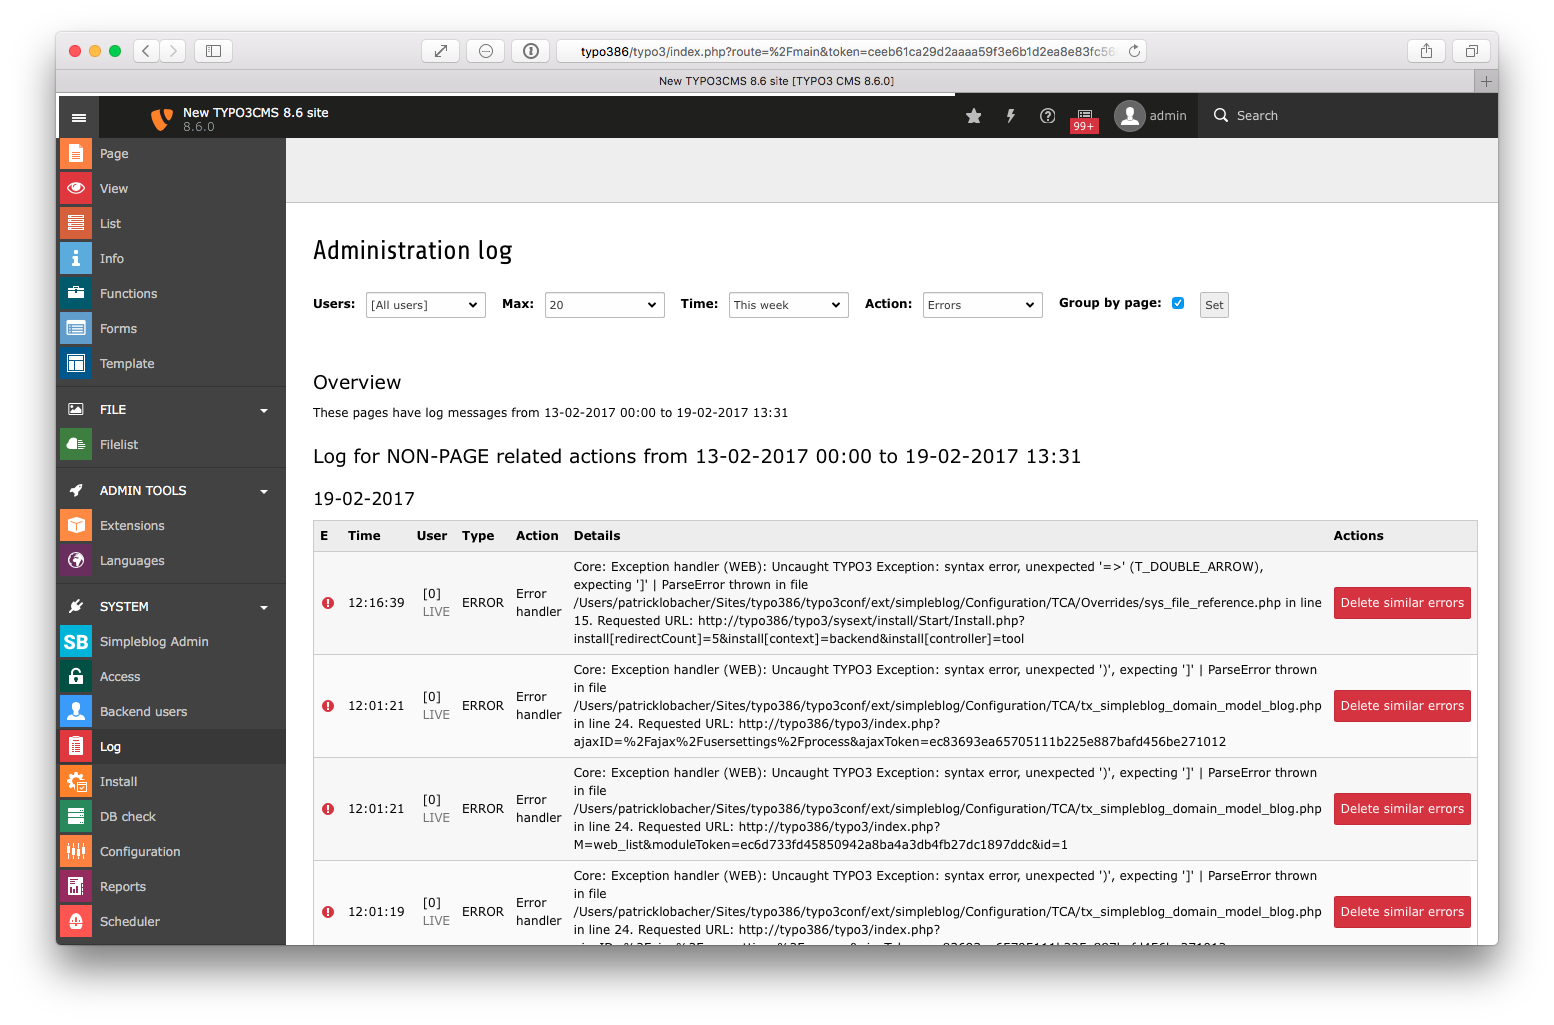
\includegraphics[width=0.60\linewidth]{BackendUserInterface/79235.png}
	\end{figure}

\end{frame}

% ------------------------------------------------------------------------------
% LTXE-SLIDE-START
% LTXE-SLIDE-UID:		8c44b86d-ce1e452e-574b316c-83250bf6
% LTXE-SLIDE-ORIGIN:	fc878ad9-7b163d51-e579b8b3-9cbe41d9 English
% LTXE-SLIDE-TITLE:		#79467: Form settings button
% LTXE-SLIDE-REFERENCE:	!Feature: #79467 - EXT:form - add form settings button to module header
% ------------------------------------------------------------------------------
\begin{frame}[fragile]
	\frametitle{Backend User Interface}
	\framesubtitle{\texttt{EXT:form}: add form settings button to module header}

	A new button has been added to the module header of the form editor.
	Clicking on this button shows the form settings within the inspector.

	\begin{figure}\vspace{-0.2cm}
		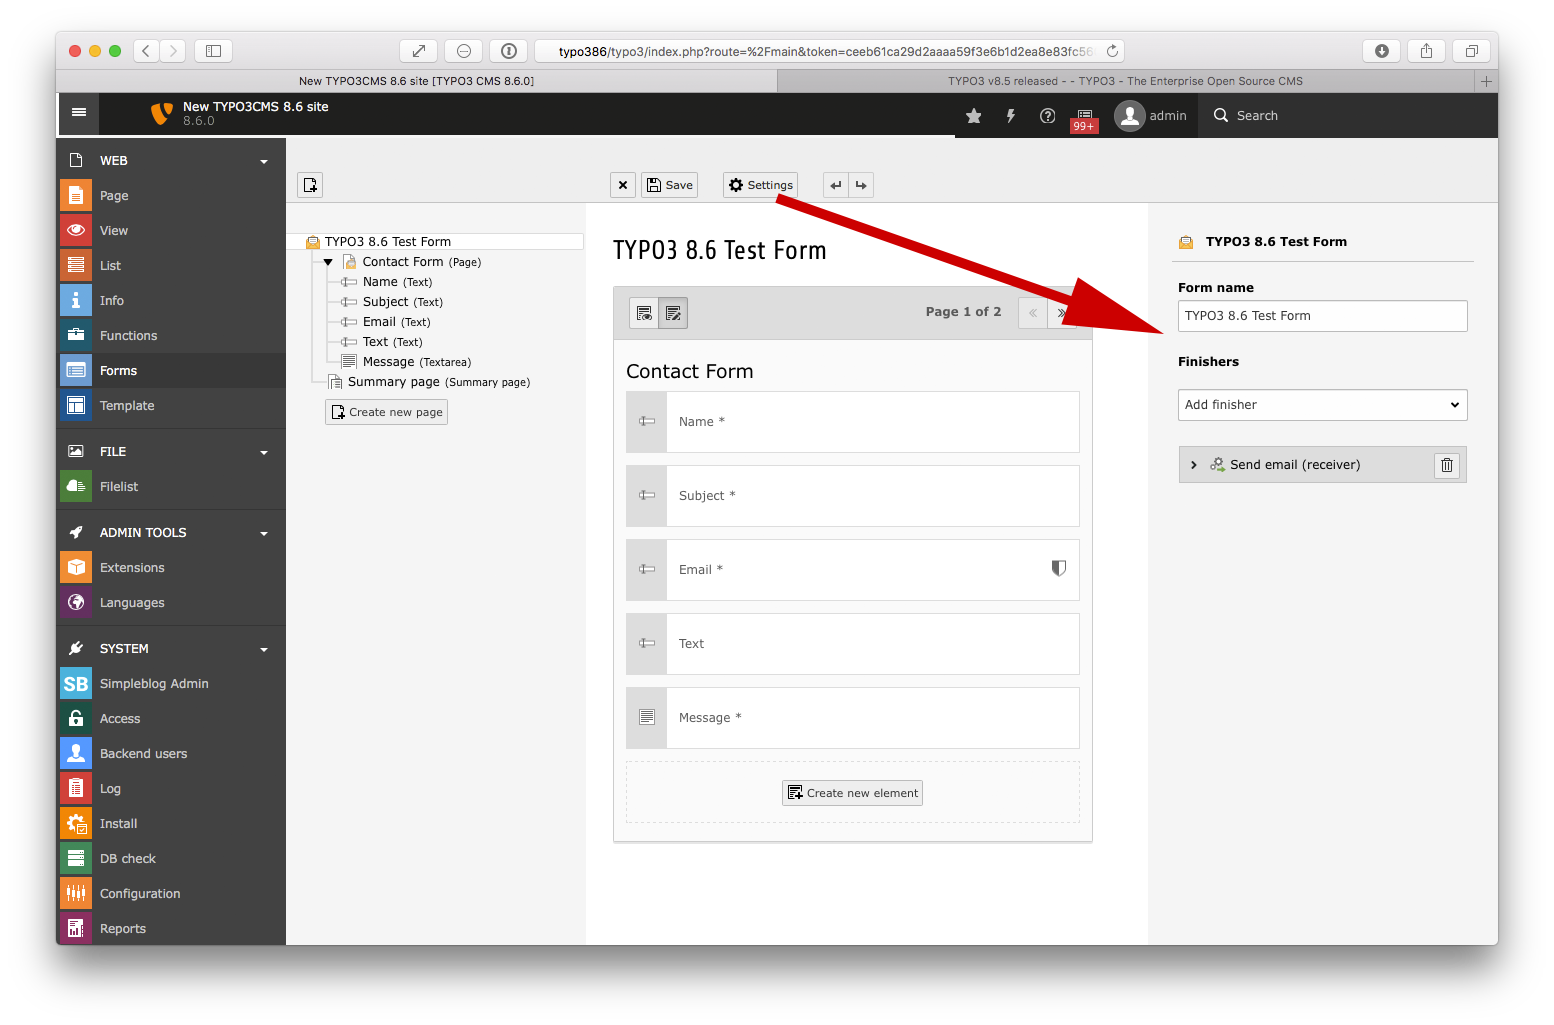
\includegraphics[width=0.675\linewidth]{BackendUserInterface/79467.png}
	\end{figure}

\end{frame}

% ------------------------------------------------------------------------------
% LTXE-SLIDE-START
% LTXE-SLIDE-UID:		af71c12e-10c61fc7-8e73955c-1a9a2db4
% LTXE-SLIDE-ORIGIN:	e1759d2e-8cc138ca-40ce6a34-65354b0e English
% LTXE-SLIDE-TITLE:		#79531: EXT:form - Add multiselect inspector editor
% LTXE-SLIDE-REFERENCE:	!Feature: #79531 - EXT:form - Add multiselect inspector editor
% ------------------------------------------------------------------------------
\begin{frame}[fragile]
	\frametitle{Backend User Interface}
	\framesubtitle{{EXT:form}: Add multiselect inspector editor}

	\begin{columns}[T]
		\begin{column}{0.35\textwidth}
			A new inspector editor, i.e. a new field type of the form editor, has been added.
			If applied, multi-select fields can be added to the inspector.
			A multi-select field allows the selection of multiple meta properties for a field
			and stores them in the defined property path.
		\end{column}

		\begin{column}{0.65\textwidth}
			\begin{figure}\vspace*{-0.6cm}
				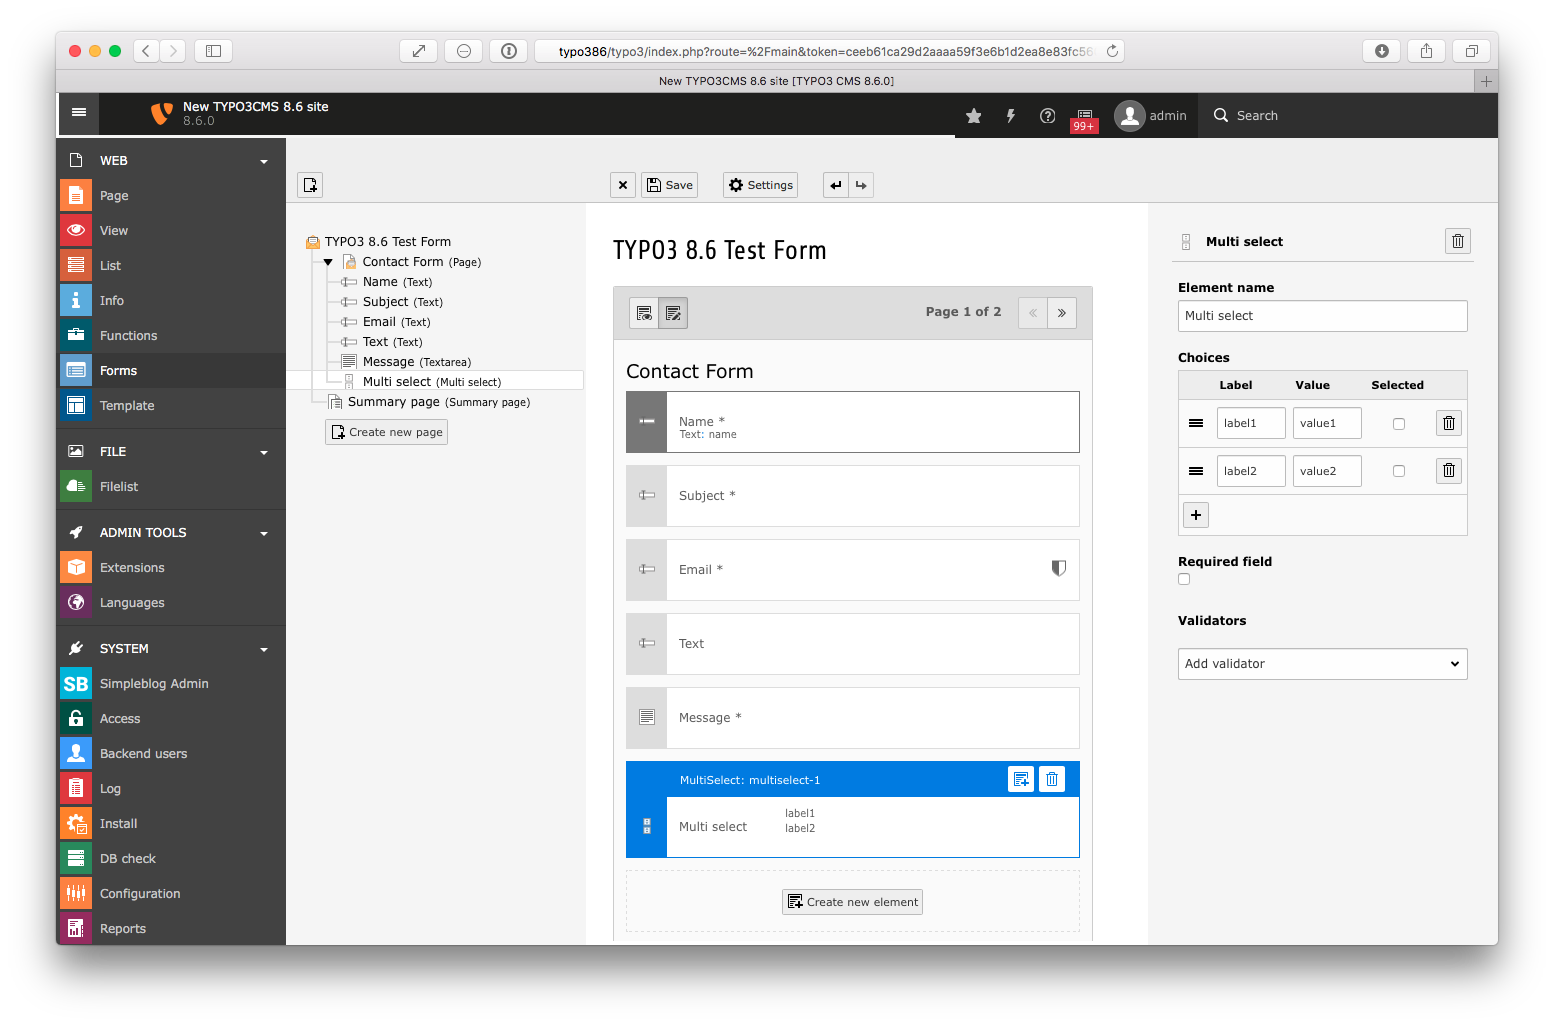
\includegraphics[width=0.99\linewidth]{BackendUserInterface/79531.png}
			\end{figure}
		\end{column}
	\end{columns}

\end{frame}

% ------------------------------------------------------------------------------
% LTXE-SLIDE-START
% LTXE-SLIDE-UID:		2cc1efd2-1b9fed47-419a1f96-4e7481f9
% LTXE-SLIDE-ORIGIN:	f6756002-b9aac45f-9460b472-1da819b5 English
% LTXE-SLIDE-TITLE:		#79521: Show list of failed input elements in FormEngine
% LTXE-SLIDE-REFERENCE:	!Feature: #79521 - Show list of failed input elements in FormEngine
% ------------------------------------------------------------------------------
\begin{frame}[fragile]
	\frametitle{Backend User Interface}
	\framesubtitle{Show list of failed input elements in FormEngine}

	\begin{columns}[T]
		\begin{column}{.35\textwidth}
			When validating input fields of the FormEngine fails, a button is now rendered into
			the button bar in the module document header. Clicking the button renders a list of
			all input elements whose validation failed. Clicking onto a field in that list
			automatically focuses the field in the form.
		\end{column}

		\begin{column}{.65\textwidth}
			\begin{figure}\vspace*{-0.6cm}
				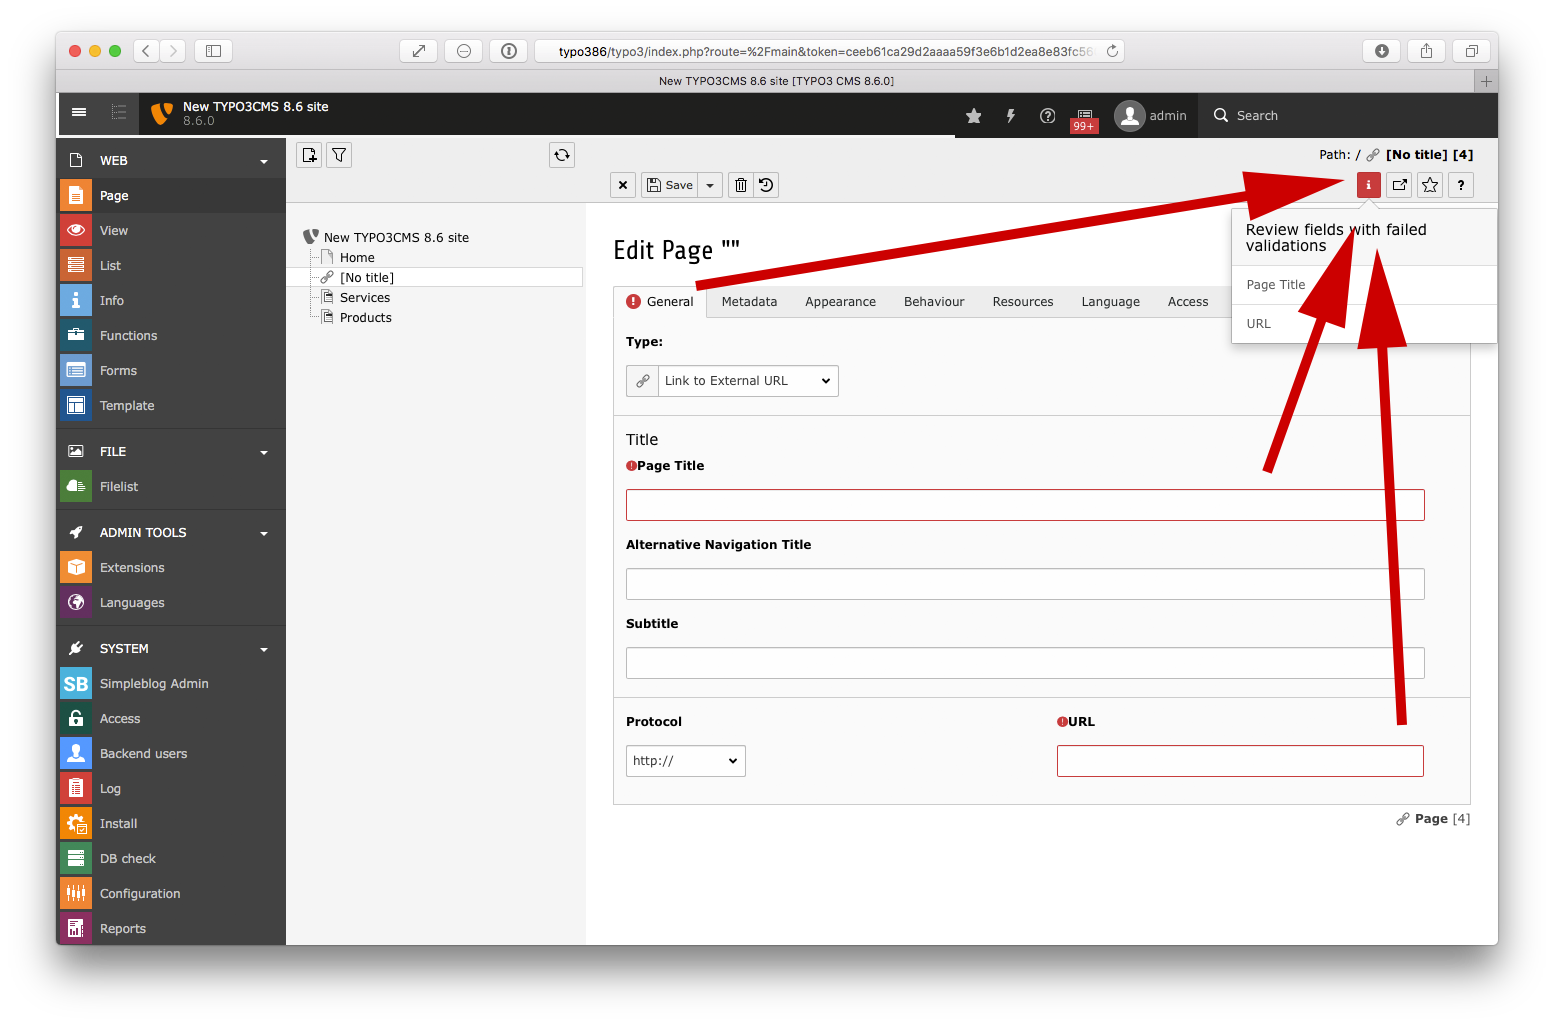
\includegraphics[width=0.99\linewidth]{BackendUserInterface/79521.png}
			\end{figure}
		\end{column}
	\end{columns}

\end{frame}

% ------------------------------------------------------------------------------
% LTXE-SLIDE-START
% LTXE-SLIDE-UID:		88420052-699dbdd1-a095ddbc-89cb01af
% LTXE-SLIDE-ORIGIN:	749a055b-02003192-92f2631e-39abcc95 English
% LTXE-SLIDE-TITLE:		#79622: Dedicated content elements for menus
% LTXE-SLIDE-REFERENCE:	!Breaking: #79622 - Dedicated content elements for menus
% ------------------------------------------------------------------------------
\begin{frame}[fragile]
	\frametitle{Backend User Interface}
	\framesubtitle{Dedicated content elements for menus}

	For better maintainability the currently existing content element menu has been
	split into dedicated content elements.

	\begin{figure}\vspace{-0.2cm}
		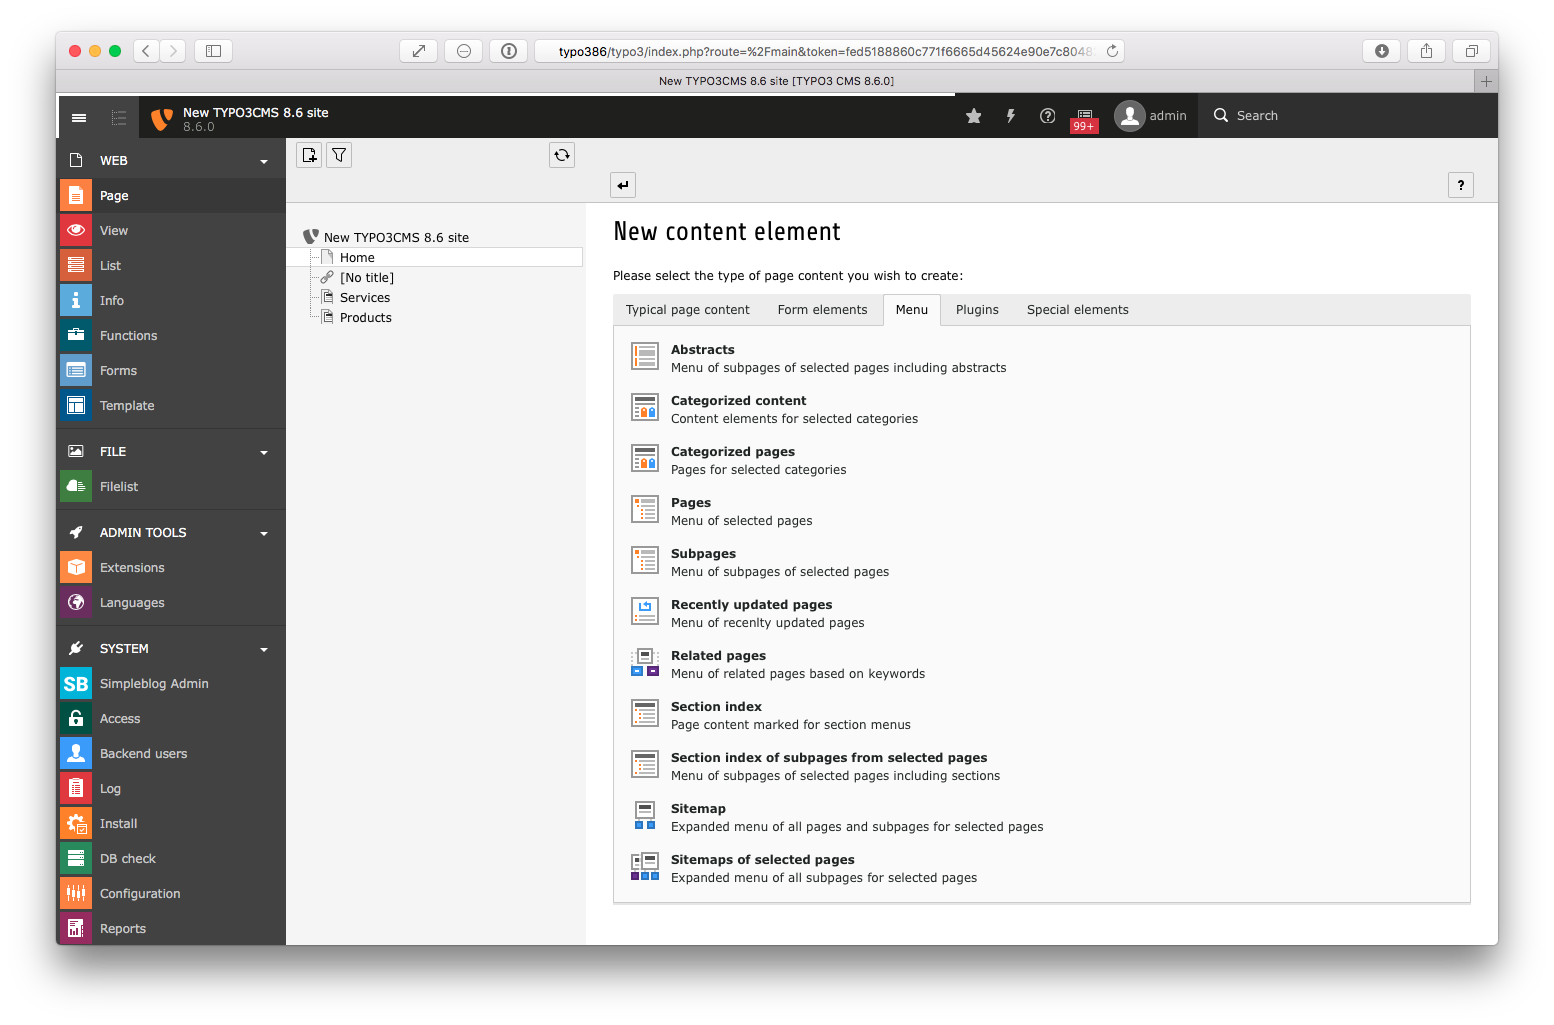
\includegraphics[width=0.68\linewidth]{BackendUserInterface/79622.png}
	\end{figure}

\end{frame}

% ------------------------------------------------------------------------------
